\documentclass[pdftex,12pt,a4paper]{article}
% can use a4 paper instead, twocolumn


% \usepackage[landscape, margin=1.5cm]{geometry}
\usepackage{graphicx}
\usepackage{listings}
%\usepackage{fullpage}
%\usepackage[usenames,dvipsnames]{xcolor}	% different hilight colors
%\usepackage{fancyhdr} % used for footer

% used to import title page
\newcommand{\HRule}{\rule{\linewidth}{0.5mm}}


\newcommand{\hilight}[1]{\colorbox{yellow}{#1}}
\newcommand{\hilightblue}[1]{\colorbox{blue}{#1}}

\begin{document}

\begin{center}
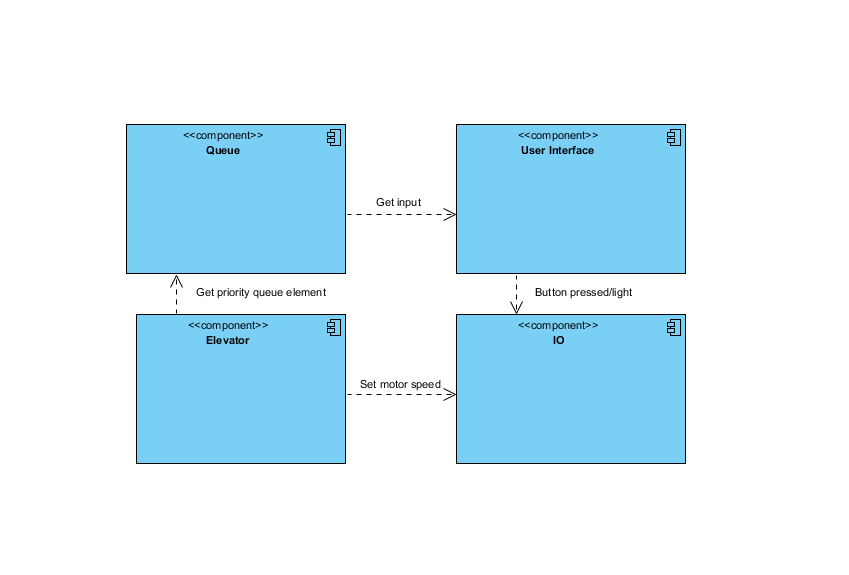
\includegraphics[scale=0.7]{./overordnet_diagram.jpg}
\\Overordnet system arkitektur
\end{center}

\begin{center}
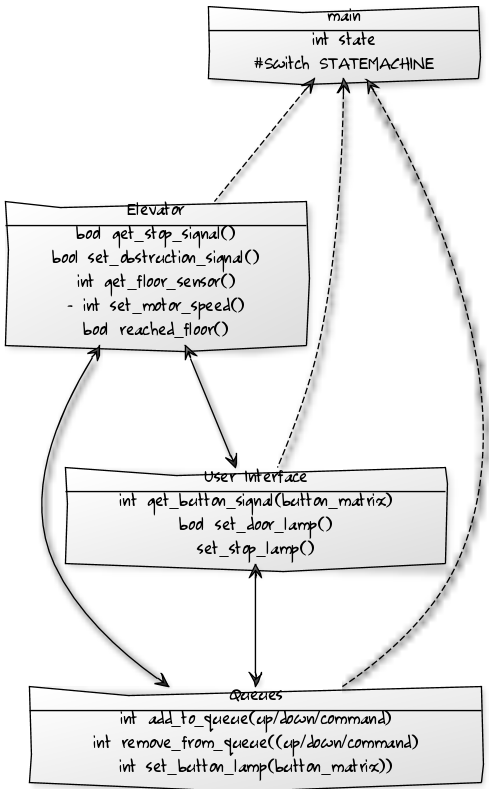
\includegraphics[scale=0.71]{./class_diagram.png}
\\Klasse diagram (I/O klasse eksludert men UI og Elevator depender på den)
\end{center}

\begin{center}
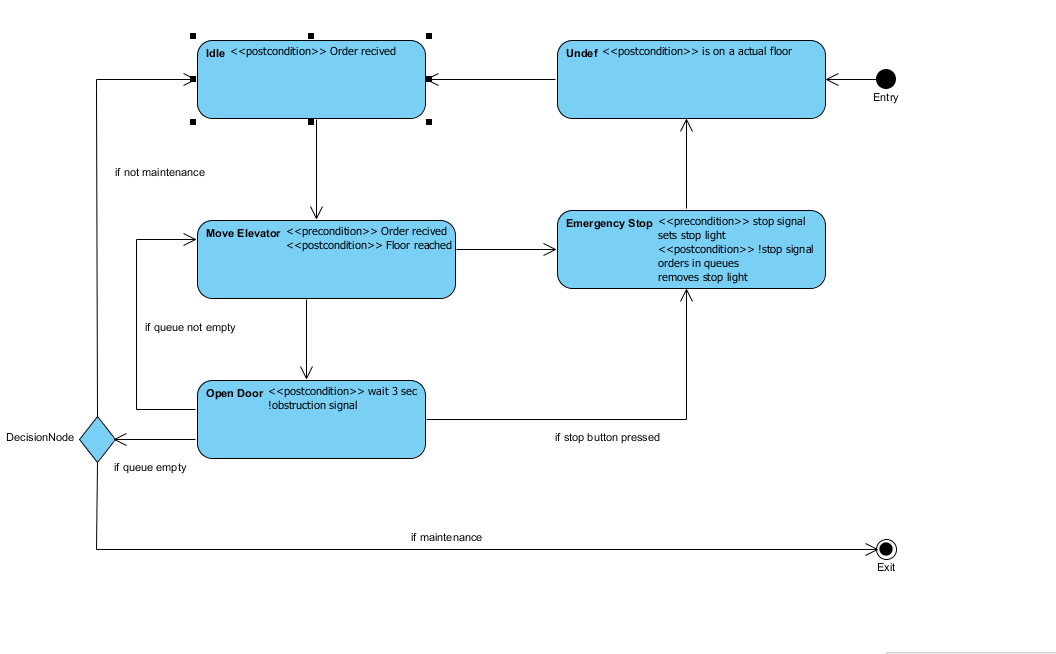
\includegraphics[scale=0.71]{./activity_diagram.png}
\\Aktivitetsdiagram
\end{center}

\begin{center}
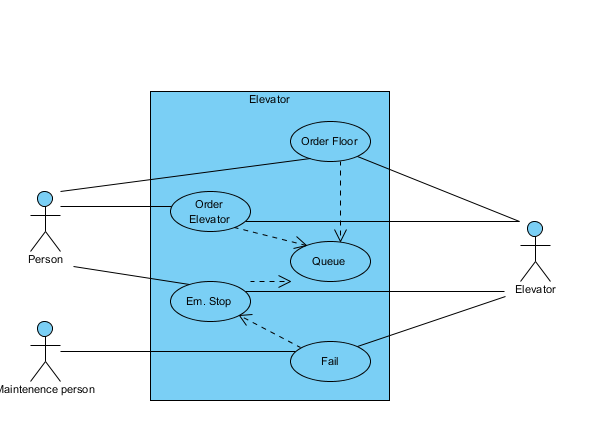
\includegraphics[scale=0.71]{./use_case_diagram.jpg}
\\Use case diagram
\end{center}


\end{document}
